% Prezentacja - etap 2 (21.X): architektura, prototypy i struktury danych.
% Kompilacja (XeLaTeX):  tectonic prezentacja.tex   albo   latexmk -xelatex prezentacja.tex
\documentclass[aspectratio=169,11pt]{beamer}

\usetheme[progressbar=frametitle,numbering=fraction]{metropolis}
\usepackage[polish]{babel}
\usepackage{booktabs}
\usepackage{tabularx}
\usepackage{listings}
\usepackage{xcolor}
\usepackage{tikz}
\usetikzlibrary{arrows.meta,positioning}

\graphicspath{{../diagramy/}{../mockup/}}
\newcolumntype{L}{>{\raggedright\arraybackslash}X}

\definecolor{ok}{HTML}{11804B}
\definecolor{bad}{HTML}{C0392B}
\definecolor{warn}{HTML}{A15C00}
\definecolor{acc}{HTML}{1F5EFF}
\newcommand{\good}[1]{\textcolor{ok}{#1}}
\newcommand{\bad}[1]{\textcolor{bad}{#1}}

\lstset{
  basicstyle=\ttfamily\footnotesize,
  keywordstyle=\color{acc}\bfseries,
  commentstyle=\color{gray},
  language=SQL,
  morekeywords={RETURNING,NOWAIT},
  columns=fullflexible,
  keepspaces=true,
  frame=none,
  backgroundcolor=\color{black!4},
  xleftmargin=4pt, framexleftmargin=4pt,
  extendedchars=true,
}

\title{System zapisów na zajęcia -- USOSv2}
\subtitle{Etap 2: architektura, prototypy i struktury danych}
\author{Kamil Kręcigłowa \and Bartosz Królik \and Krzysztof Krówka}
\institute{Inżynieria Oprogramowania, zima 2026/2027}
\date{21 października 2026}

\begin{document}

\maketitle

% ---------------------------------------------------------------------------
\begin{frame}{Temat i plan prezentacji}
  \begin{columns}[T]
    \begin{column}{0.52\textwidth}
      \textbf{Temat 2: System zapisu na zajęcia}
      \begin{itemize}\small
        \item ograniczona liczba miejsc, różne rozmiary grup
        \item katalog: kursy, grupy, prowadzący, harmonogram
        \item wymagania wstępne (zaliczone przedmioty)
        \item wykrywanie kolizji w planie
        \item listy oczekujących z automatycznym zapisem
      \end{itemize}
    \end{column}
    \begin{column}{0.42\textwidth}
      \textbf{Plan}
      \begin{enumerate}\small
        \item Architektura i stos technologiczny
        \item Przypadki użycia
        \item Struktury danych (ER)
        \item Prototypy obszarów ryzyka
        \item Mock-up interfejsu
      \end{enumerate}
    \end{column}
  \end{columns}
\end{frame}

\begin{frame}{Pokrycie wymagań}
  \footnotesize
  \begin{tabularx}{\textwidth}{@{}>{\raggedright}p{3.4cm}>{\raggedright}p{2.4cm}L>{\raggedright\arraybackslash}p{1.8cm}@{}}
    \toprule
    \textbf{Wymaganie} & \textbf{Przypadki} & \textbf{Tabele (ER)} & \textbf{Prototyp} \\
    \midrule
    ograniczona liczba miejsc & UC2, UC13 & \texttt{section.capacity}, \texttt{enrolled\_count}, \texttt{waitlist\_limit} & scen. 1, 5 \\
    katalog i harmonogram & UC1, UC11, UC12 & \texttt{course}, \texttt{section}, \texttt{section\_lecturer}, \texttt{meeting}, \texttt{room}, \texttt{term}, \texttt{enrollment\_round} & scen. 6 \\
    różne rozmiary grup & UC12, UC13 & \texttt{section.capacity}, \texttt{section.kind}, \texttt{room.seats} & scen. 1, 4, 5 \\
    wymagania wstępne & UC3, UC11, UC15 & \texttt{course\_prerequisite}, \texttt{completed\_course} & scen. 2, 6 \\
    kolizje w harmonogramie & UC4, UC12 & \texttt{meeting} (dzień, godziny, parzystość) & scen. 3 \\
    listy oczekujących & UC5, UC7, UC9, UC18 & \texttt{waitlist\_entry}, \texttt{notification} & scen. 4, 5, 6 \\
    \bottomrule
  \end{tabularx}
\end{frame}

% ---------------------------------------------------------------------------
\section{Architektura}

\begin{frame}[plain]
  \begin{tikzpicture}[remember picture, overlay]
    \node at (current page.center) {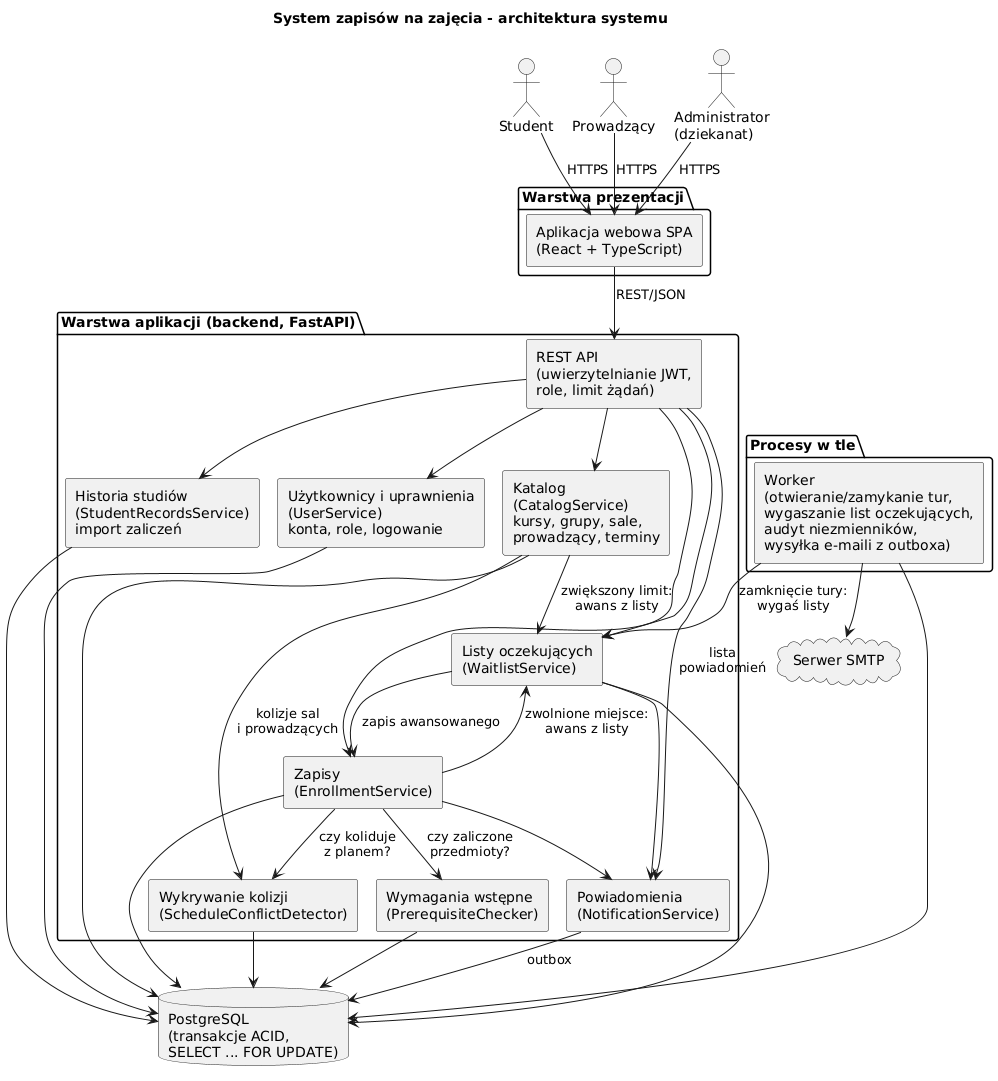
\includegraphics[height=0.98\paperheight]{architektura.png}};
  \end{tikzpicture}
\end{frame}

\begin{frame}{Architektura: moduły i odpowiedzialności}
  \begin{columns}[T]
    \begin{column}{0.5\textwidth}
      \small
      \begin{itemize}
        \item \textbf{SPA} (React + TS) dla trzech ról
        \item \textbf{REST API} (FastAPI): JWT, role, limit żądań
        \item \texttt{EnrollmentService} -- \emph{jedyny} moduł zmieniający liczbę zajętych miejsc
        \item \texttt{PrerequisiteChecker}, \texttt{ScheduleConflictDetector} -- reguły zapisu
        \item \texttt{WaitlistService} -- kolejka i automatyczny awans
        \item \texttt{NotificationService} -- outbox w bazie
      \end{itemize}
    \end{column}
    \begin{column}{0.46\textwidth}
      \small
      \begin{itemize}
        \item \textbf{Worker}: otwiera i zamyka tury, wygasza listy, audytuje niezmienniki, wysyła e-maile
        \item \textbf{PostgreSQL} -- jedno źródło prawdy
      \end{itemize}
      \begin{alertblock}{Główne wyzwanie}
        Otwarcie tury: setki studentów naraz walczą o te same miejsca.
        Zapis do grupy serializuje blokada jej wiersza, a zapisy studenta -- blokada wiersza studenta.
      \end{alertblock}
    \end{column}
  \end{columns}
\end{frame}

\begin{frame}{Stos technologiczny}
  \small
  \begin{tabularx}{\textwidth}{@{}l>{\raggedright}p{4.4cm}L@{}}
    \toprule
    \textbf{Element} & \textbf{Technologia} & \textbf{Uzasadnienie} \\
    \midrule
    Frontend & React + TypeScript & typowanie, łatwy katalog, formularze, siatka planu \\
    Backend & Python 3.12, FastAPI, SQLAlchemy & szybkie prototypowanie, OpenAPI, walidacja (Pydantic), async \\
    Baza danych & PostgreSQL 16 & ACID, blokady wierszy, indeksy częściowe, \texttt{TIME}, \texttt{JSONB} \\
    Zadania w tle & własny worker (APScheduler) & outbox i tury w bazie -- broker zbędny \\
    Uwierzytelnianie & JWT, docelowo SSO uczelni & bezstanowe API, proste role \\
    Wdrożenie & Docker Compose & to samo środowisko dla całego zespołu \\
    \bottomrule
  \end{tabularx}
\end{frame}

% ---------------------------------------------------------------------------
\section{Przypadki użycia}

\begin{frame}{Przypadki użycia (1/2): student}
  \centering
  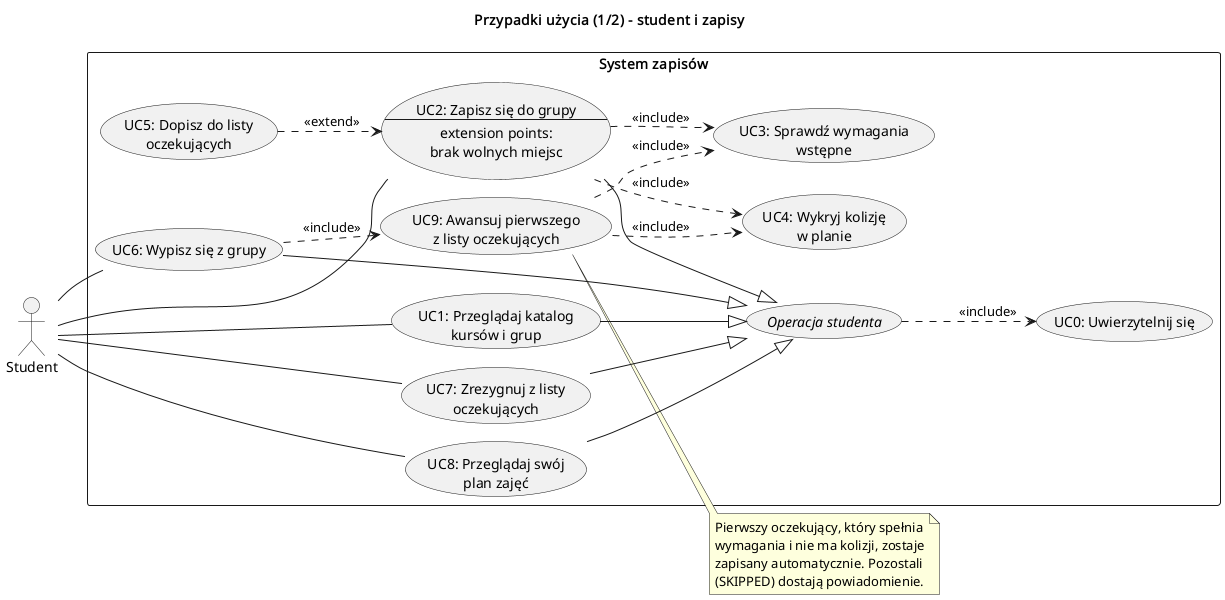
\includegraphics[height=0.86\textheight,width=\textwidth,keepaspectratio]{przypadki_uzycia_student.png}
\end{frame}

\begin{frame}{Przypadki użycia (2/2): dziekanat, prowadzący, zegar}
  \centering
  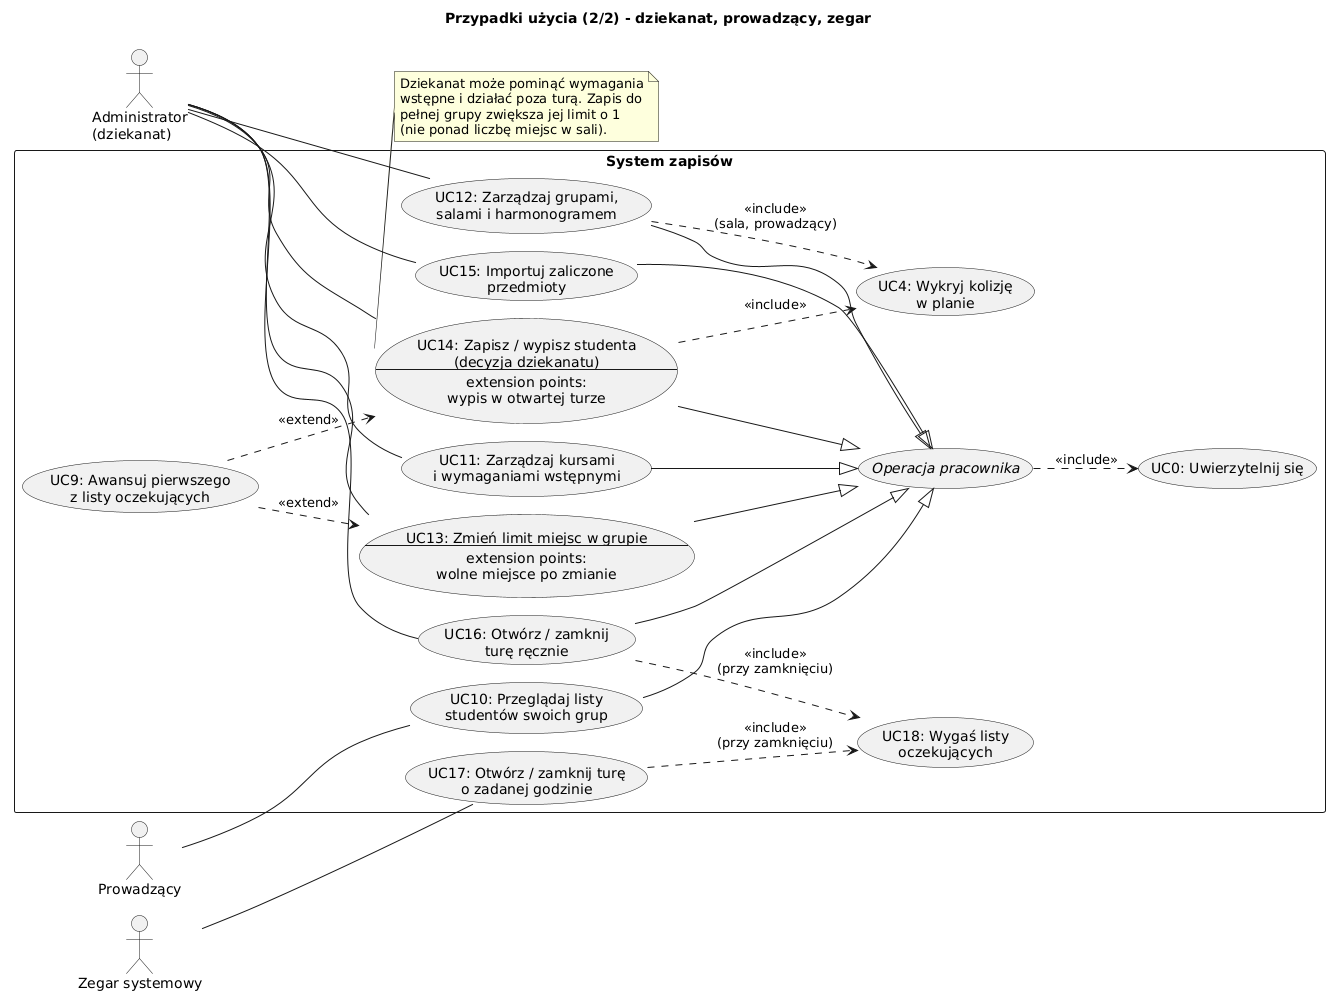
\includegraphics[height=0.86\textheight,width=\textwidth,keepaspectratio]{przypadki_uzycia_administracja.png}
\end{frame}

\begin{frame}{UC2: Zapisz się do grupy}
  \begin{columns}[T]
    \begin{column}{0.5\textwidth}
      \small
      \textbf{Przebieg główny}
      \begin{enumerate}
        \item Student wybiera grupę z katalogu (UC1).
        \item Blokada wiersza \textbf{studenta}, potem \textbf{grupy}.
        \item Wymagania wstępne (UC3).
        \item Kolizje z planem (UC4).
        \item Wolne miejsce $\Rightarrow$ zapis, licznik $+1$;
              wpisy na listach innych grup tego przedmiotu i typu $\Rightarrow$ CANCELLED.
        \item Grupa pojawia się w planie (UC8).
      \end{enumerate}
    \end{column}
    \begin{column}{0.46\textwidth}
      \small
      \textbf{Scenariusze alternatywne (odmowa z przyczyną)}
      \begin{itemize}
        \item brak zaliczenia / kolizja (który przedmiot, która grupa)
        \item już ma grupę tego przedmiotu i typu (wykład + lab -- wolno)
        \item już zapisany lub już czeka na tę grupę
        \item tura zamknięta
        \item brak miejsc $\Rightarrow$ \textbf{UC5} (\texttt{<<extend>>}): koniec listy, o ile nie przekroczono \texttt{waitlist\_limit}
      \end{itemize}
    \end{column}
  \end{columns}
\end{frame}

\begin{frame}{UC9: Awans z listy oczekujących}
  \setlength{\itemsep}{0pt}
  \begin{columns}[T]
    \begin{column}{0.55\textwidth}
      \small
      Wywoływany w \textbf{tej samej transakcji}, która zwolniła miejsce:
      wypis (UC6), zmiana limitu (UC13), decyzja dziekanatu (UC14).
      \begin{enumerate}
        \item Dopóki jest wolne miejsce -- bierz pierwszego \texttt{WAITING}.
        \item Sprawdź \textbf{ponownie} wymagania, kolizje i regułę ,,jedna grupa danego typu''.
        \item Spełnia $\Rightarrow$ zapis (\texttt{source = WAITLIST}) i powiadomienie.
        \item Nie spełnia $\Rightarrow$ \texttt{SKIPPED} z powodem, powiadomienie, następny.
      \end{enumerate}
    \end{column}
    \begin{column}{0.41\textwidth}
      \small
      \textbf{Decyzje projektowe}
      \begin{itemize}
        \item bez wolnego miejsca nikogo nie pomijamy -- student może jeszcze usunąć kolizję
        \item zamknięcie tury (UC16/UC17) $\Rightarrow$ UC18: listy wygasają (\texttt{EXPIRED})
        \item dziekanat (UC14): może pominąć wymagania i działać poza turą;
              zapis do pełnej grupy = limit $+1$ (max. liczba miejsc w sali)
      \end{itemize}
      \begin{exampleblock}{Niezmiennik}
        Nikt nie czeka na liście, gdy w grupie są wolne miejsca.
      \end{exampleblock}
    \end{column}
  \end{columns}
\end{frame}

% ---------------------------------------------------------------------------
\section{Struktury danych}

\begin{frame}[plain]
  \begin{tikzpicture}[remember picture, overlay]
    \node at (current page.center) {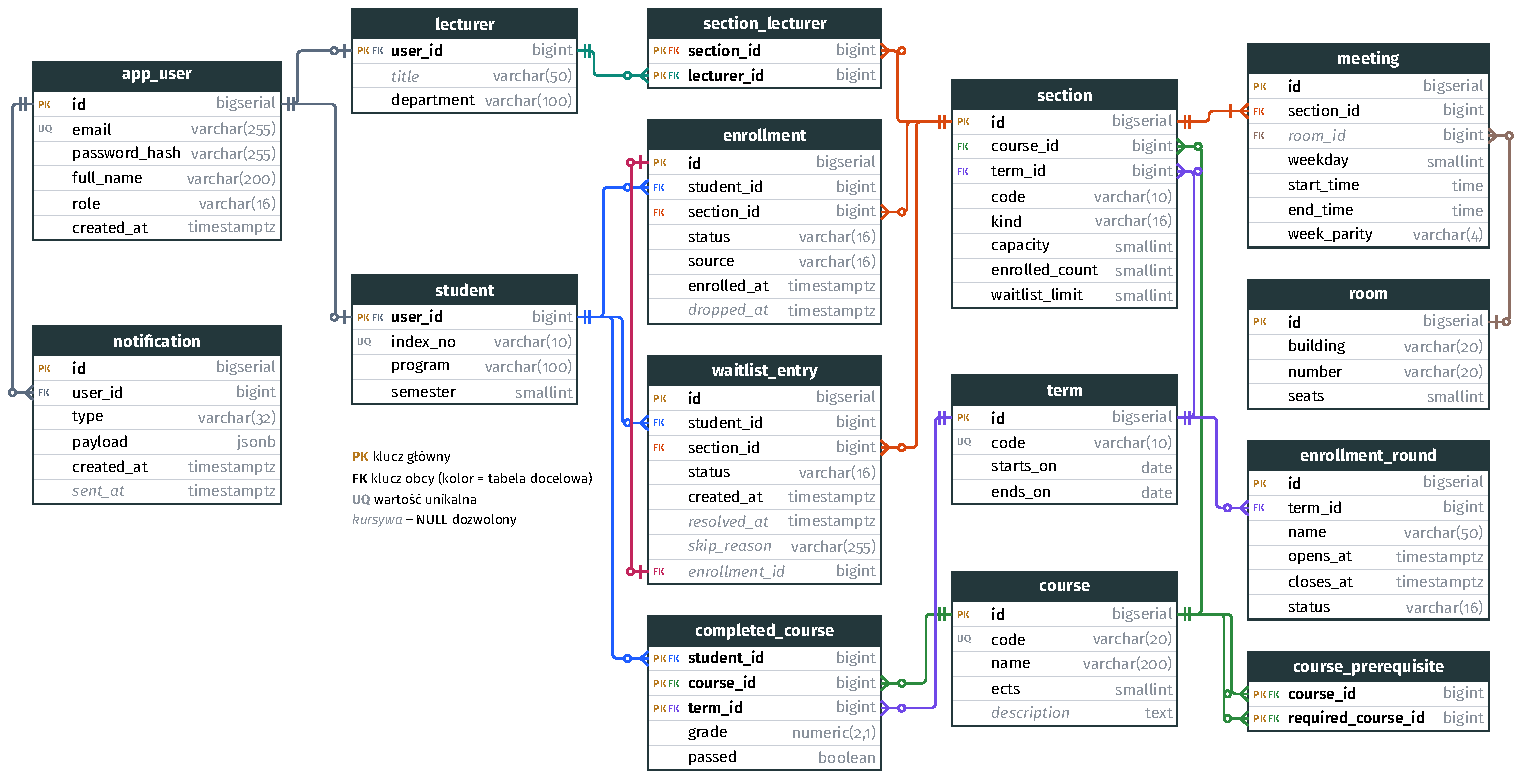
\includegraphics[width=0.99\paperwidth,height=0.98\paperheight,keepaspectratio]{er.pdf}};
  \end{tikzpicture}
\end{frame}

\begin{frame}{Najważniejsze decyzje w modelu danych}
  \begin{columns}[T]
    \begin{column}{0.5\textwidth}
      \small
      \begin{itemize}
        \item \textbf{Kurs $\neq$ grupa}: \texttt{course} w katalogu, \texttt{section} w semestrze z własnym limitem i typem
        \item \textbf{Harmonogram} w \texttt{meeting}: dzień, godziny, parzystość tygodni semestru, sala
        \item \textbf{Licznik} \texttt{enrolled\_count}: sprawdzenie limitu i zajęcie miejsca to jeden \texttt{UPDATE}
        \item \textbf{Historia zamiast kasowania}: \texttt{DROPPED}, \texttt{PROMOTED}, \texttt{SKIPPED}, \texttt{CANCELLED}, \texttt{EXPIRED}
      \end{itemize}
    \end{column}
    \begin{column}{0.46\textwidth}
      \small
      \begin{itemize}
        \item \textbf{Indeksy częściowe}: jeden aktywny zapis / wpis na liście
        \item \textbf{Kolejność listy} = \texttt{id} z sekwencji (nadawane pod blokadą grupy)
        \item \textbf{Tury} w \texttt{enrollment\_round}, najwyżej jedna otwarta w semestrze
        \item \texttt{passed} wyliczane z oceny, trigger blokuje cykle wymagań
        \item \textbf{Outbox}: powiadomienie w tej samej transakcji co awans
      \end{itemize}
    \end{column}
  \end{columns}
\end{frame}

\begin{frame}[fragile]{Reguła kolizji}
  \begin{columns}[T]
    \begin{column}{0.52\textwidth}
      \small
      Dwa terminy kolidują, gdy:
      \begin{itemize}
        \item ten sam dzień tygodnia,
        \item godziny się przecinają (styk końcem \emph{nie} koliduje),
        \item tygodnie się pokrywają: \texttt{ALL} -- ze wszystkim, \texttt{ODD} -- z \texttt{ODD}, \texttt{EVEN} -- z \texttt{EVEN},
        \item ten sam semestr.
      \end{itemize}
\begin{lstlisting}[basicstyle=\ttfamily\scriptsize]
mine.weekday = other.weekday
AND mine.start_time < other.end_time
AND other.start_time < mine.end_time
AND (mine.week_parity = 'ALL'
  OR other.week_parity = 'ALL'
  OR mine.week_parity = other.week_parity)
\end{lstlisting}
    \end{column}
    \begin{column}{0.44\textwidth}
      \small
      Plan: pon 10:00--11:30,\\ śr 12:00--13:30 (tyg. nieparzyste)\\[4pt]
      \begin{tabular}{@{}lr@{}}
        \toprule
        \textbf{Nowa grupa} & \textbf{Wynik} \\
        \midrule
        pon 11:00--12:30 & \bad{KOLIZJA} \\
        pon 11:30--13:00 (styk) & \good{ok} \\
        wt 10:00--11:30 & \good{ok} \\
        śr 12:00--13:30 parzyste & \good{ok} \\
        śr 13:00--14:30 co tydzień & \bad{KOLIZJA} \\
        \bottomrule
      \end{tabular}\\[4pt]
      \footnotesize Funkcja SQL \texttt{schedule\_conflicts(student, grupa)}.
    \end{column}
  \end{columns}
\end{frame}

% ---------------------------------------------------------------------------
\section{Prototypy}

\begin{frame}{Obszary ryzyka i prototyp}
  \begin{columns}[T]
    \begin{column}{0.55\textwidth}
      \small
      \begin{enumerate}
        \item \textbf{Wyścig o ostatnie miejsca} (\emph{check-then-act})
        \item \textbf{Wymagania wstępne}
        \item \textbf{Kolizje} -- styk końcem, tygodnie parzyste
        \item \textbf{Automatyczny zapis z listy}: każde miejsce zajęte raz, kolejność, pomijanie niespełniających warunków
        \item Jedna grupa danego typu, limit listy, ponowny zapis
        \item Decyzje dziekanatu, zamknięcie tury
      \end{enumerate}
    \end{column}
    \begin{column}{0.41\textwidth}
      \small
      \texttt{prototyp/prototyp\_zapisow.py}
      \begin{itemize}
        \item Python + SQLite, tylko biblioteka standardowa
        \item równoległe wątki z barierą
        \item \texttt{check\_invariants()} po każdym scenariuszu
      \end{itemize}
      Schemat docelowy (\texttt{schemat.sql}) sprawdzony na \textbf{PostgreSQL~16}.
    \end{column}
  \end{columns}
\end{frame}

\begin{frame}[fragile]{Scenariusz 1: 30 studentów, 10 miejsc}
  \begin{columns}[T]
    \begin{column}{0.53\textwidth}
      \small
      Transakcja zapisu (\texttt{READ COMMITTED}):
\begin{lstlisting}
BEGIN;
SELECT 1 FROM app_user
 WHERE id = :s AND role = 'STUDENT'
   FOR UPDATE;
SELECT ... FROM section
 WHERE id = :g FOR UPDATE;
-- tura, wymagania, kolizje
UPDATE section
   SET enrolled_count = enrolled_count + 1
 WHERE id = :g
   AND enrolled_count < capacity;
INSERT INTO enrollment ...
COMMIT;
\end{lstlisting}
      Wynik: 10 zapisanych, 20 na liście.
    \end{column}
    \begin{column}{0.43\textwidth}
      \small
      30 transakcji do jednej grupy:
      \begin{itemize}
        \item blokadę grupy ma jedna, reszta czeka,
        \item każda następna widzi licznik po \texttt{COMMIT} poprzedniej,
        \item jedenasta dostaje 0 wierszy z \texttt{UPDATE} i trafia na listę oczekujących.
      \end{itemize}
      Blokada studenta: jego dwa równoległe zapisy nie sprawdzą kolizji jednocześnie.\\[4pt]
      \footnotesize Bez blokad prototyp zapisał 30 osób przy liczniku równym 1.
    \end{column}
  \end{columns}
\end{frame}

\begin{frame}{Scenariusze 4--6: lista oczekujących}
  \small
  \begin{itemize}
    \item L01 pełna (2/2), czekają: 3, 4, 5, 6. Student 3 zapisuje się na kolidujące BD L05.
    \item Limit bez zmian $\Rightarrow$ nikt nie awansuje, student 3 \good{nadal czeka}.
    \item Student 1 się wypisuje $\Rightarrow$ 3: \texttt{SKIPPED} (kolizja z L05), 4: \texttt{PROMOTED}.
    \item Dwa wypisy w tej samej chwili $\Rightarrow$ awansują dokładnie dwaj pierwsi, kolejność zachowana.
    \item Piotr czeka na L03 i zapisuje się na L05 $\Rightarrow$ wpis na L03 \texttt{CANCELLED}, zwolnione miejsce na liście dostaje Kuba.
    \item Ponowny zapis do tej samej grupy $\Rightarrow$ odmowa (,,już zapisany'' / ,,już czeka'').
    \item Dziekanat zapisuje Ewę bez wymagań do pełnej L07 $\Rightarrow$ limit $2 \to 3$, Kuba nadal czeka.
    \item Zamknięcie tury $\Rightarrow$ lista wygasa; wypis po turze przez dziekanat nikogo nie zapisuje.
  \end{itemize}
  \begin{exampleblock}{}
    Wszystkie niezmienniki spełnione po każdym kroku.
  \end{exampleblock}
\end{frame}

\begin{frame}[fragile]{Blokady w PostgreSQL: zakleszczenie przy awansie}
  \begin{columns}[T]
    \begin{column}{0.52\textwidth}
      \centering
      \begin{tikzpicture}[
          node distance=6mm,
          tx/.style={draw, rounded corners, minimum width=26mm, minimum height=7mm, font=\footnotesize, align=center},
          res/.style={draw, fill=black!6, minimum width=20mm, minimum height=7mm, font=\footnotesize},
          >={Stealth}]
        \node[tx] (t1) {Wypis A\\+ awans B};
        \node[tx, right=26mm of t1] (t2) {Zapis B\\do tej grupy};
        \node[res, below=12mm of t1] (sec) {grupa};
        \node[res, below=12mm of t2] (stB) {student B};
        \draw[->, ok, thick] (sec) -- node[left, font=\scriptsize]{trzyma} (t1);
        \draw[->, ok, thick] (stB) -- node[right, font=\scriptsize]{trzyma} (t2);
        \draw[->, bad, thick, dashed] (t1.south east) -- (stB.north west) node[pos=0.8, above right, font=\scriptsize]{czeka};
        \draw[->, bad, thick, dashed] (t2.south west) -- (sec.north east) node[pos=0.8, above left, font=\scriptsize]{czeka};
      \end{tikzpicture}\\[6pt]
      \raggedright\small
      Zapis blokuje studenta, potem grupę. Awans: grupę, potem studenta B.\\[3pt]
      Przy zwykłym \texttt{FOR UPDATE} PostgreSQL po \texttt{deadlock\_timeout} (1~s) przerywa jedną z transakcji błędem 40P01 (sprawdzone na PostgreSQL~16).
    \end{column}
    \begin{column}{0.44\textwidth}
      \small
      Awans blokuje B bez czekania:
\begin{lstlisting}
SELECT 1 FROM app_user
 WHERE id = :b AND role = 'STUDENT'
   FOR UPDATE NOWAIT;
\end{lstlisting}
      Zajęty B: od razu błąd 55P03, wypis się wycofuje i jest ponawiany.\\[4pt]
      Awans zostaje w tej samej transakcji co zwolnienie miejsca, więc nikt spoza listy go nie zajmie, a B nie traci kolejki.\\[3pt]
      \footnotesize 40P01 i 40001 obsługujemy tak samo.
    \end{column}
  \end{columns}
\end{frame}

% ---------------------------------------------------------------------------
\section{Mock-up}

\begin{frame}{Mock-up: ekran zapisów studenta}
  \begin{columns}[T]
    \begin{column}{0.6\textwidth}
      \centering
      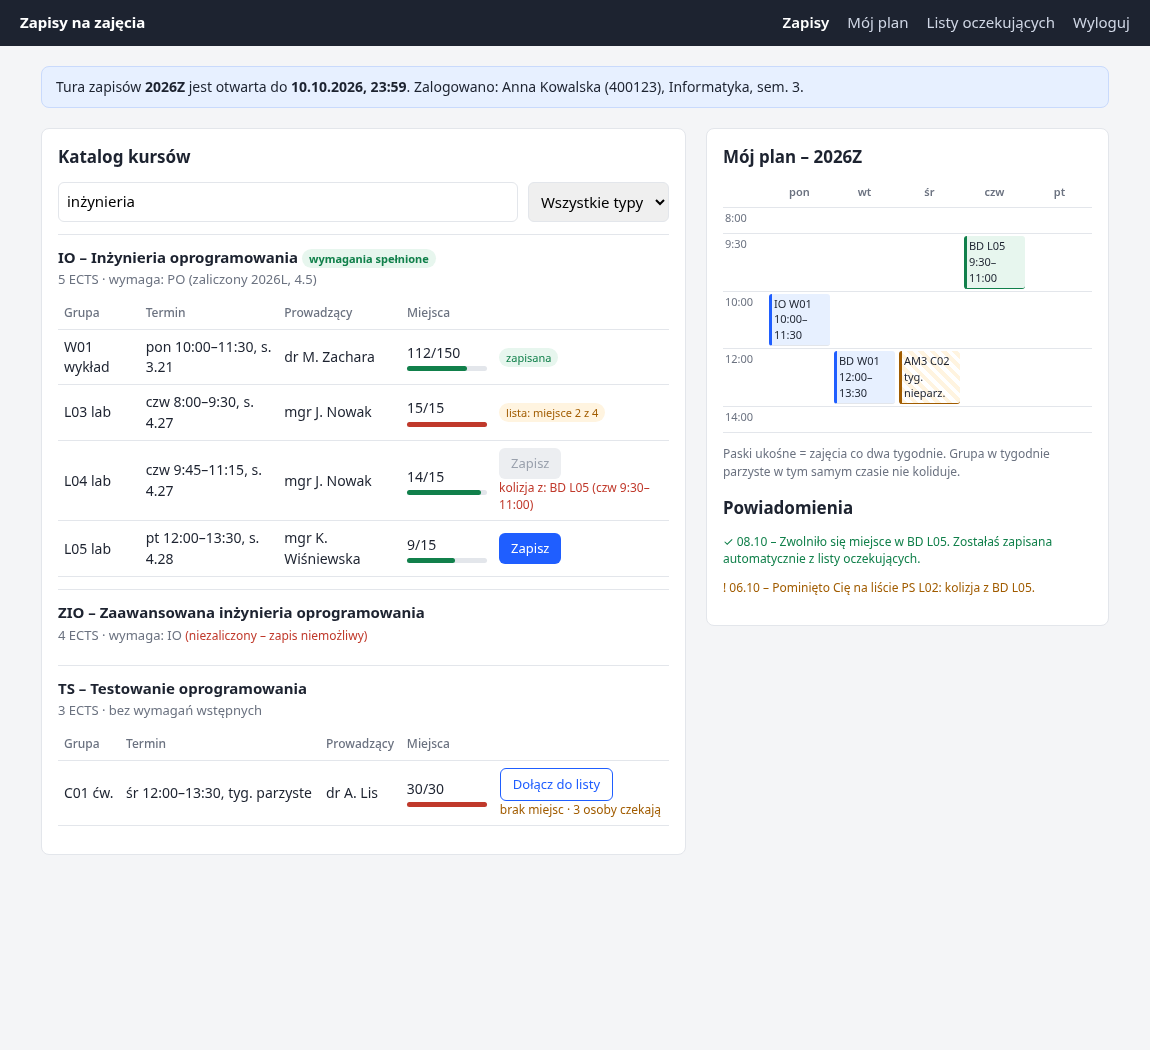
\includegraphics[height=0.84\textheight]{mockup.png}
    \end{column}
    \begin{column}{0.38\textwidth}
      \footnotesize
      \begin{itemize}
        \item katalog z zajętością miejsc
        \item kurs zablokowany przez niezaliczony przedmiot
        \item ,,Zapisz'' zablokowane przez kolizję, z podaniem grupy
        \item pozycja na liście, ,,Zrezygnuj'', ,,Dołącz do listy''
        \item ostrzeżenie: zapis usunie z listy innej grupy
        \item plan tygodnia z zajęciami co dwa tygodnie
        \item powiadomienia o awansie i pominięciu
      \end{itemize}
    \end{column}
  \end{columns}
\end{frame}

\begin{frame}[standout]
  Dziękujemy!\\[6pt]
  \normalsize Pytania?
\end{frame}

\end{document}
